% main.tex - IEEE conference format (IEEEtran). Build: pdflatex main; bibtex main; pdflatex main x2
% Every number in the text comes from numbers.tex, generated by analysis/analyze.py.
% Lines marked TODO are unfinished and must not survive into the submitted version.
\documentclass[conference]{IEEEtran}
\usepackage{cite,amsmath,graphicx,booktabs,xspace,url}
\usepackage[hidelinks]{hyperref}
% generated by analysis/analyze.py - do not edit by hand
\newcommand{\NumAnswers}{380\xspace}
\newcommand{\NumTimedRuns}{10{,}358\xspace}
\newcommand{\NumPowerOffset}{0.49\xspace}
\newcommand{\NumHwQueries}{1\xspace}
% --- extended numbers ---
\newcommand{\NumOrigAnswers}{282\xspace}
\newcommand{\NumFbAnswers}{83\xspace}
\newcommand{\NumHwxAnswers}{15\xspace}
\newcommand{\NumAllAnswers}{380\xspace}
\newcommand{\NumTimedRunsAll}{18{,}629\xspace}
\newcommand{\NumCorrectGemma}{93\xspace}
\newcommand{\NumAdaptGemmaPlain}{42\xspace}
\newcommand{\NumAdaptGemmaHw}{100\xspace}
\newcommand{\NumCorrectFlash}{100\xspace}
\newcommand{\NumAdaptFlashPlain}{0\xspace}
\newcommand{\NumAdaptFlashHw}{100\xspace}
\newcommand{\NumCorrectChatgpt}{90\xspace}
\newcommand{\NumAdaptChatgptPlain}{43\xspace}
\newcommand{\NumAdaptChatgptHw}{46\xspace}
\newcommand{\NumCorrectDeepseek}{87\xspace}
\newcommand{\NumAdaptDeepseekPlain}{43\xspace}
\newcommand{\NumAdaptDeepseekHw}{31\xspace}
\newcommand{\NumCorrectClaude}{100\xspace}
\newcommand{\NumAdaptClaudePlain}{40\xspace}
\newcommand{\NumAdaptClaudeHw}{93\xspace}
\newcommand{\NumCorrectDsapi}{87\xspace}
\newcommand{\NumAdaptDsapiPlain}{45\xspace}
\newcommand{\NumAdaptDsapiHw}{51\xspace}
\newcommand{\NumHwQueriesAll}{1\xspace}
\newcommand{\NumPChatgpt}{0.3394\xspace}
\newcommand{\NumPClaude}{0.0010\xspace}
\newcommand{\NumPDeepseek}{0.5771\xspace}
\newcommand{\NumPDsapi}{0.5250\xspace}
\newcommand{\NumPFlash}{1.0000\xspace}
\newcommand{\NumPGemma}{0.0014\xspace}
\newcommand{\NumStaticUniMin}{2\xspace}
\newcommand{\NumStaticUniMax}{23\xspace}
\newcommand{\NumStaticMildMin}{6\xspace}
\newcommand{\NumStaticMildMax}{14\xspace}
\newcommand{\NumStaticHistogram}{23\xspace}
\newcommand{\NumStaticKmeans}{18\xspace}
\newcommand{\NumStaticNorm}{13\xspace}
\newcommand{\NumAdaptIrregular}{98\xspace}
\newcommand{\NumAdaptUniform}{2\xspace}
\newcommand{\NumStaticMandel}{109\xspace}
\newcommand{\NumStaticTrisum}{63\xspace}
\newcommand{\NumShortcutPlain}{5\xspace}
\newcommand{\NumShortcutNPlain}{6 of 129\xspace}
\newcommand{\NumShortcutHw}{6\xspace}
\newcommand{\NumShortcutNHw}{8 of 128\xspace}
\newcommand{\NumShortcutFb}{32\xspace}
\newcommand{\NumShortcutNFb}{24 of 75\xspace}
\newcommand{\NumShortcutHwx}{21\xspace}
\newcommand{\NumShortcutNHwx}{3 of 14\xspace}
\newcommand{\NumFbPairs}{83\xspace}
\newcommand{\NumFbBoth}{75\xspace}
\newcommand{\NumFbStaticTotal}{44\xspace}
\newcommand{\NumFbStaticToAdapt}{1\xspace}
\newcommand{\NumFbScaleRatio}{0.97\xspace}
\newcommand{\NumFbScaleP}{0.05\xspace}
\newcommand{\NumFbBestRatio}{1.25\xspace}
\newcommand{\NumFbBestP}{0.03\xspace}
\newcommand{\NumFbBroken}{8\xspace}
\newcommand{\NumFbFixed}{0\xspace}
\newcommand{\NumReproWithinOne}{14\xspace}
\newcommand{\NumReproMaxDev}{6\xspace}
\newcommand{\NumOrigCompile}{15\xspace}
\newcommand{\NumOrigCrash}{2\xspace}
\newcommand{\NumOrigWrong}{2\xspace}
\newcommand{\NumOrigNoCode}{6\xspace}
\newcommand{\NumWzeroMin}{0.95\xspace}
\newcommand{\NumWzeroMax}{1.13\xspace}
\newcommand{\NumAdaptPlainMin}{40\xspace}
\newcommand{\NumAdaptPlainMax}{43\xspace}
\newcommand{\NumShortcutRatio}{6\xspace}
\newcommand{\NumLpmMin}{1.9\xspace}
\newcommand{\NumLpmMax}{2.4\xspace}
\newcommand{\NumCollectFrom}{20\xspace}
\newcommand{\NumCollectTo}{23 Nov 2026\xspace}
\newcommand{\NumSwitchUpGemma}{23\xspace}
\newcommand{\NumSwitchDownGemma}{0\xspace}
\newcommand{\NumSwitchPGemma}{<0.0001\xspace}
\newcommand{\NumSwitchUpClaude}{8\xspace}
\newcommand{\NumSwitchDownClaude}{0\xspace}
\newcommand{\NumSwitchPClaude}{0.008\xspace}
\newcommand{\NumSwitchUpChatgpt}{0\xspace}
\newcommand{\NumSwitchDownChatgpt}{0\xspace}
\newcommand{\NumSwitchPChatgpt}{n/a\xspace}
\newcommand{\NumSwitchUpDeepseek}{0\xspace}
\newcommand{\NumSwitchDownDeepseek}{0\xspace}
\newcommand{\NumSwitchPDeepseek}{n/a\xspace}
\newcommand{\NumSwitchUpDsapi}{4\xspace}
\newcommand{\NumSwitchDownDsapi}{1\xspace}
\newcommand{\NumSwitchPDsapi}{0.375\xspace}

% generated by analysis/figures.py - do not edit by hand
\newcommand{\NumPlaceSerialP}{0.95\xspace}
\newcommand{\NumPlaceFourP}{3.55\xspace}
\newcommand{\NumPlaceFourE}{0.13\xspace}
\newcommand{\NumPlaceSixE}{1.90\xspace}
\newcommand{\NumPlaceTenE}{5.31\xspace}
\newcommand{\NumPlaceTenP}{3.59\xspace}
\newcommand{\NumOverMandelbrotTen}{2.09\xspace}
\newcommand{\NumOverMandelbrotTwenty}{1.36\xspace}
\newcommand{\NumOverTrisumTen}{1.63\xspace}
\newcommand{\NumOverTrisumTwenty}{1.15\xspace}
\newcommand{\NumMandelJSerial}{5.3\xspace}
\newcommand{\NumMandelJStatic}{3.4\xspace}
\newcommand{\NumMandelJDyn}{1.1\xspace}
\newcommand{\NumCalibKernels}{5\xspace}
\newcommand{\NumCalibSlowerMin}{3\xspace}
\newcommand{\NumCalibSlowerMax}{22\xspace}
\newcommand{\NumCalibSlowerCount}{5\xspace}

\newcommand{\todo}[1]{\textbf{\textcolor{red}{[TODO: #1]}}}
\usepackage{xcolor}

\begin{document}
\title{Heterogeneity-Blind? Evaluating LLM-Generated OpenMP Code on an Asymmetric P/E-Core Processor}
\author{\IEEEauthorblockN{Mohamed Qurrain Shayeeb\textsuperscript{*}, Dr.\ Mallegowda M\textsuperscript{\dag}}
\IEEEauthorblockA{Department of Computer Science and Engineering\\
Ramaiah Institute of Technology, Bangalore, India\\
\textsuperscript{*}qsirius12@gmail.com \qquad \textsuperscript{\dag}mallegowda@msrit.edu}}
\maketitle

\begin{abstract}
Large language models are increasingly used to parallelize code, but no evaluation of LLM-generated OpenMP that we know of measures it on a processor whose cores run at different speeds. Consumer processors now mix fast performance (P) cores with slower efficiency (E) cores. We present the first study of LLM-generated OpenMP on such a processor: \NumAllAnswers{} answers from five LLM families (four vendors) for 15 C kernels, measured on an Apple M4 (4P+6E) with \NumTimedRunsAll{} timed runs and per-core activity and energy sampled during every run. No answer queried the core topology, and only one of \NumAllAnswers{} requested thread binding, even when the prompt described the hardware. The models nonetheless avoid most of the asymmetry penalty by habit, choosing adaptive schedules for visibly irregular loops; the residual cost falls on uniform loops, where static schedules run up to \NumStaticUniMax\% slower once threads spill onto E-cores. Describing the hardware changed the schedules of two models and not the others. Measurement feedback fixed none of the asymmetry and made work-removing shortcuts about \NumShortcutRatio{} times more common. The standard remedy for asymmetric processors, a start-up-calibrated static split, was slower than plain adaptive scheduling on every kernel we tried, because macOS migrates threads between core types. We release all prompts, answers, timings and scripts.
\end{abstract}

\begin{IEEEkeywords}
large language models, OpenMP, code generation, asymmetric multicore, heterogeneous cores, loop scheduling, Apple Silicon, energy
\end{IEEEkeywords}

%=====================================================================
\section{Introduction}
Large language models (LLMs) are now routinely asked to parallelize code, and a growing body of work evaluates how well they write OpenMP~\cite{nichols2024pareval,chen2024ompgpt,mahmud2025autoparllm,kadosh2024ompar}. None of these evaluations measures the code on a P/E hybrid processor. Consumer and laptop processors, however, are no longer homogeneous: Intel's hybrid chips and every Apple Silicon processor mix fast performance (P) cores with slower, more efficient (E) cores. On such processors the default assumption behind a static loop partition---that every thread finishes its equal share at the same time---is false, work on asymmetric multicore processors (AMPs), a long-studied scheduling problem~\cite{david2017amp}, shows that conventional OpenMP schedules leave fast cores idle~\cite{saez2020aid}. Intel's own library guide recommends running threads on the P-cores only, because splitting work across both core types is hard to balance~\cite{intel2025mkl}.

This raises a question nobody has measured: \emph{when an LLM parallelizes a loop, does it account for cores of unequal speed, and what does it cost when it does not?} The closest prior work studies one hand-written Monte Carlo kernel on an Intel hybrid processor~\cite{beserra2026amp}; the closest LLM work compares generated code across CPU architectures, none of them a P/E hybrid~\cite{codegenbench2026}.

We answer the question on an Apple M4 (4\,P\,+\,6\,E cores, macOS), where the operating system---not the program---decides thread placement through quality-of-service classes~\cite{eclectic2022m1sched}, so thread pinning is unavailable. We ask:
\begin{itemize}
\item \textbf{RQ1:} Do LLMs account for core asymmetry when they parallelize serial C code with OpenMP?
\item \textbf{RQ2:} How much performance does LLM-generated code lose relative to the best schedule an expert could choose?
\item \textbf{RQ3:} Does describing the hardware in the prompt, or explicitly asking for E-core-aware code, change the code they write?
\item \textbf{RQ4:} Does measurement feedback let them close the remaining gap?
\end{itemize}

\textbf{Contributions.}
(1)~The first empirical study of LLM-generated OpenMP on a performance-asymmetric processor: \NumAllAnswers{} answers from five LLM families from four vendors (six access paths) on 15 kernels, \NumTimedRunsAll{} timed runs.
(2)~Direct evidence of where threads ran, from per-core activity sampled during every run, together with per-run CPU energy.
(3)~A taxonomy separating heterogeneity-blind scheduling, compiler failures and algorithmic shortcuts, with a two-factor speedup decomposition that keeps shortcuts from masquerading as good parallelization.
(4)~An evaluation of hardware-aware prompting and measurement feedback against expert schedules, including an AID-style calibrated split~\cite{saez2020aid}.
(5)~All prompts, raw replies, timings, power logs and scripts, released for reproduction. \todo{repository URL and DOI}

%=====================================================================
\section{Background and Related Work}
\subsection{LLMs for parallel code}
ParEval~\cite{nichols2024pareval} showed that LLMs do markedly worse on parallel than on serial problems and that correct parallel code is often inefficient. Specialized models generate OpenMP pragmas~\cite{chen2024ompgpt}, graph-based analysis can guide an LLM to the loops worth parallelizing~\cite{mahmud2025autoparllm}, retrieval improves pragma validity~\cite{abdullah2025p4omp}, and learned source-to-source tools outperform rule-based auto-parallelizers~\cite{kadosh2024ompar}. Reinforcement learning from performance feedback produces faster code~\cite{nichols2024rlpf}, and recent studies evaluate task-based~\cite{bantel2026tasks} and MPI+OpenMP code~\cite{diehl2026llmhpc}. CodegenBench~\cite{codegenbench2026} evaluates generated parallel code on x86-64, Sunway and Kunpeng processors, but none of these is a P/E hybrid on which the operating system places ordinary threads on cores of unequal speed. Benchmark contamination~\cite{chen2025dycodeeval} and multi-dimensional scoring~\cite{pcebench2025} inform our methodology.

\subsection{OpenMP on asymmetric processors}
On AMPs, static schedules hand slow cores as much work as fast ones, and dynamic schedules pay a coordination cost. AID~\cite{saez2020aid} distributes iterations in proportion to measured core speed inside the runtime and improves on static and dynamic scheduling by up to 56\% and 16.8\%. On an Intel Core i5-1235U, standard OpenMP schedules suffer load imbalance on a Monte Carlo kernel and calibration-based splits improve runtime~\cite{beserra2026amp}, while a study of thread pinning on an Intel Alder Lake processor finds no single best policy~\cite{sscad_pinning}. Machine-learned optimization heuristics can choose such parameters but are typically trained for each target platform~\cite{wang2018mlcompiler}. These approaches target human-written code or the runtime; none examines what LLMs produce.

\subsection{Apple Silicon}
The M4 has four P-cores and six E-cores. macOS places threads by quality-of-service class: lowest-QoS threads run only on E-cores, and higher-QoS work fills P-cores first and then spills onto E-cores~\cite{eclectic2022m1sched,eclectic2021m1perf}. OpenMP's binding controls therefore have no effect. Peer-reviewed measurements of this behaviour are scarce~\cite{lviv2025applesched}; Section~\ref{sec:placement} contributes direct per-core evidence.

%=====================================================================
\section{Methodology}\label{sec:method}
\subsection{Kernels}
% generated by analysis/analyze.py - do not edit by hand
\begin{table}[t]\centering\caption{Kernels (serial time: median of five runs).}\label{tab:kernels}
\footnotesize\setlength{\tabcolsep}{3pt}\begin{tabular}{@{}lllr@{}}\toprule
Kernel & Computation & Cost & Serial (s) \\\midrule
saxpy & y=ax+y, repeated & unif., mem.-bound & 0.80 \\
matmul & dense matrix product & uniform & 1.10 \\
jacobi2d & 5-point stencil sweeps & unif., mem.-bound & 0.67 \\
trisum & triangular row sums & irregular & 0.96 \\
mandelbrot & escape-time iteration & irregular & 1.41 \\
spmv & sparse mat.-vec., skewed rows & irregular & 0.84 \\
nbody & all-pairs forces & uniform & 0.79 \\
histogram & 256-bin histogram, repeated & uniform & 0.79 \\
norm & sum of sqrt$|x|$, repeated & uniform & 0.76 \\
prefix & inclusive prefix sum & loop-carried & 0.39 \\
primes & prime count, trial division & irregular & 0.92 \\
collatz & Collatz step counts & irregular & 1.11 \\
conv2d & 2-D convolution, 15$\times$15 & uniform & 1.12 \\
kmeans & Lloyd's k-means & uniform & 1.11 \\
cutoff & neighbours within radius & irregular & 1.07 \\
\bottomrule\end{tabular}\end{table}

Table~\ref{tab:kernels} lists the fifteen kernels: six with uniform per-iteration cost, six irregular, two memory-bound and one with a loop-carried dependency. Input sizes were chosen so that each serial run takes about one second.
Each kernel is a complete C program whose parallelizable region lies between two markers. Inputs are generated by a fixed-seed xorshift generator so that every variant sees identical data; correctness is checked against the serial checksum (exact for integer kernels, relative tolerance $10^{-9}$ for floating point, $10^{-6}$ for two count kernels with floating-point boundary tests).

\subsection{Models and prompts}
\begin{table}[t]\centering\caption{Models and access paths (answers collected \NumCollectFrom--\NumCollectTo).}\label{tab:models}
\footnotesize\setlength{\tabcolsep}{3pt}\begin{tabular}{@{}lp{5.0cm}c@{}}\toprule
Model & Access and settings & Samples \\\midrule
Gemma 4 31B & Gemini API, default settings & 3 \\
Gemini 3.8 Flash & Gemini API (free tier, partial) & 1--3 \\
ChatGPT & chatgpt.com, Go plan, default model, Think off & 1 \\
DeepSeek (web) & chat.deepseek.com, DeepThink and Search off & 1 \\
DeepSeek (API) & \texttt{deepseek-flash} (V4.1-Flash-1017), thinking disabled & 3 \\
Claude & claude.ai, Opus 5.5, default effort, incognito chat & 1 \\\bottomrule
\end{tabular}\end{table}
Web answers were collected in fresh chats, by pasting the prompt and copying the reply through each site's own controls; no prompt or reply was retyped, and every prompt was checked against a checksum of the file sent to the API models. Web interfaces do not expose an exact model version, which is why one model family (DeepSeek) was also queried through its versioned API.
Every model received byte-identical prompts in four styles: \emph{plain} (rules only), \emph{hw} (plus a description of the 4P+6E machine and the absence of pinning), \emph{hwx} (hw plus an explicit request to perform well despite the slower E-cores) and \emph{fb} (the plain prompt plus the model's own previous answer and its measured times, with no hint about the cause).

\subsection{Baselines}
Serial; an expert version with \texttt{schedule(runtime)} swept over static, dynamic (two chunk sizes per kernel class) and guided; and an AID-style calibrated split that times a fixed loop on each thread at start-up and assigns iterations in proportion to speed~\cite{saez2020aid,beserra2026amp}.

\subsection{Platform and measurement}
MacBook Air (M4, 4P+6E, 24\,GB, fanless), macOS 26, Apple clang 21 with Homebrew libomp 21.1.3 (OpenMP 5.1), flags \texttt{-O2 -ffp-contract=off}. Each configuration (variant $\times$ schedule $\times$ \{1,2,4,6,8,10\} threads) ran five times in shuffled order with a 1\,s cool-down; we report medians. CPU power and per-core activity were sampled every 250\,ms with \texttt{powermetrics}; its timestamps are truncated to whole seconds, a fixed \NumPowerOffset\,s offset we estimated by cross-correlation and corrected. All reported runs used macOS's normal power mode on mains power; an earlier session with Low Power Mode on (which slows single-thread runs by \NumLpmMin--\NumLpmMax$\times$) was kept as a separate condition and is not mixed into the results. Variants were measured over four nights, each night with its own serial and expert baselines, and every variant is compared only with baselines from its own night.

\subsection{Metrics}
For an answer with median times $T_1$ and $T_{10}$ and serial time $T_s$ we report the serial-optimization factor $F=T_s/T_1$ and the parallel scaling $S=T_1/T_{10}$, so the overall speedup $T_s/T_{10}=F\cdot S$ separates rewriting the algorithm from parallelizing it. Answers are classified by reading the code: W0 (parallelized only), W1 (work-preserving rewrite), W1c (rewrite a compiler can collapse), W2 (repeated or algorithmic work removed).

%=====================================================================
\section{Results}
\subsection{Correctness}
Of the \NumOrigAnswers{} answers to the plain and hardware prompts, Claude and Gemini Flash produced correct programs every time (\NumCorrectClaude\% and \NumCorrectFlash\%), Gemma \NumCorrectGemma\%, ChatGPT \NumCorrectChatgpt\%, DeepSeek via the web \NumCorrectDeepseek\% and via the API \NumCorrectDsapi\%. Most compile errors share one cause: code that calls \texttt{omp\_get\_thread\_num()} without including \texttt{omp.h}, which GCC accepts with a warning but Apple clang rejects. DeepSeek's failures were replies containing only fragments of \texttt{kernel()}; the remaining failures were \NumOrigCompile{} compile errors under Apple clang, \NumOrigCrash{} crash and \NumOrigWrong{} wrong result (\NumOrigNoCode{} replies had no complete program). Correctness was judged against the serial checksum after we removed one compiler effect: Apple clang~21 miscompiles the histogram kernel's per-thread bin loop at \texttt{-O2} (correct with vectorization disabled or at \texttt{-O0}, no undefined behaviour found), so every histogram variant, serial included, was built with \texttt{-fno-vectorize}.

\subsection{Where threads actually run}\label{sec:placement}
Fig.~\ref{fig:placement} shows, for long expert runs, how many core-equivalents of each type were busy. Up to four threads stay on the P-cores (\NumPlaceFourP{} P-cores and \NumPlaceFourE{} E-cores busy at four threads); from six threads macOS spills onto the E-cores, reaching \NumPlaceTenE{} busy E-cores at ten threads while the P-cores stay near \NumPlaceTenP. This is the first direct measurement we know of that confirms the P-first placement policy described informally for Apple Silicon~\cite{eclectic2021m1perf}, and it means any thread beyond the fourth runs on a slower core.

\begin{figure}[t]\centering
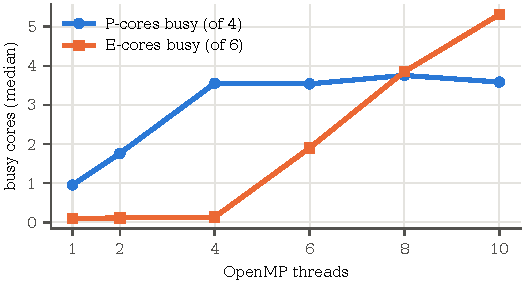
\includegraphics[width=\columnwidth]{figs/placement.pdf}
\caption{Busy cores by type during expert runs (median over runs $\geq$0.5\,s; per-core activity sampled every 250\,ms).}\label{fig:placement}
\end{figure}

\subsection{RQ1: Do LLMs account for asymmetry?}
None of the \NumAllAnswers{} answers queries the core topology or uses macOS QoS, and only \NumHwQueriesAll{} requests thread binding (a \texttt{proc\_bind(spread)} clause from DeepSeek API, which cannot take effect because macOS offers no thread affinity), even when the prompt states that the machine has four fast and six slow cores. The only asymmetry-relevant decision the models make is the schedule clause (Fig.~\ref{fig:schedules}), and they make it from the shape of the loop, not the machine: under the plain prompt they chose \texttt{dynamic} or \texttt{guided} for \NumAdaptIrregular\% of answers to irregular kernels and for \NumAdaptUniform\% of answers to uniform ones. Under the plain prompt, \NumAdaptPlainMin--\NumAdaptPlainMax\% of answers from Gemma, ChatGPT, DeepSeek and Claude use \texttt{dynamic} or \texttt{guided}; the rest use \texttt{static} explicitly or omit the clause, which in LLVM's runtime also means static. Gemini Flash used static in every plain answer.

\begin{figure}[t]\centering
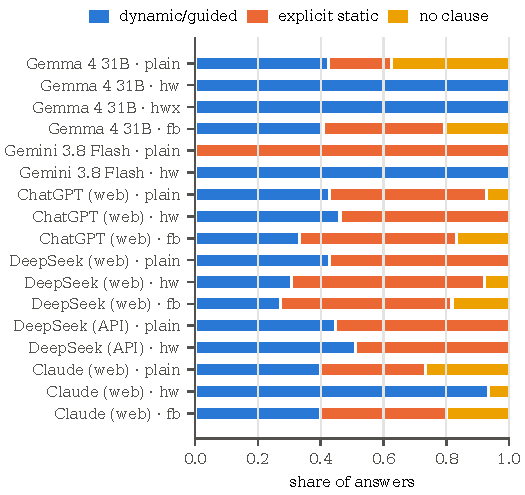
\includegraphics[width=\columnwidth]{figs/schedules.pdf}
\caption{Schedule clause chosen, by model and prompt style.}\label{fig:schedules}
\end{figure}

\subsection{RQ2: The cost of heterogeneity-blind choices}
Fig.~\ref{fig:penalty} isolates the cost of a static schedule using the expert versions. On strongly irregular kernels the penalty is large (mandelbrot \NumStaticMandel\%, trisum \NumStaticTrisum\% slower than the best schedule at ten threads) and on mildly irregular ones moderate (\NumStaticMildMin--\NumStaticMildMax\%: collatz, primes, cutoff, spmv). More telling for asymmetry, compute-bound kernels whose iterations all cost the same still lose \NumStaticUniMin--\NumStaticUniMax\% (histogram \NumStaticHistogram\%, kmeans \NumStaticKmeans\%, norm \NumStaticNorm\%): equal chunks finish at unequal times once threads land on E-cores. Memory-bound kernels (saxpy, jacobi2d) are insensitive.

\begin{figure}[t]\centering
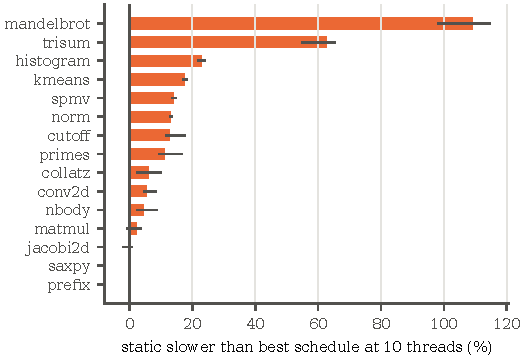
\includegraphics[width=\columnwidth]{figs/static_penalty.pdf}
\caption{Slowdown of \texttt{schedule(static)} relative to the best schedule at 10 threads (expert code; 95\% bootstrap CI over repetitions).}\label{fig:penalty}
\end{figure}

LLM answers that only add OpenMP directives (class W0) land close to the best expert schedule on average (Fig.~\ref{fig:vsbest}): geometric means lie between \NumWzeroMin{} and \NumWzeroMax{} of the expert's speed, because the kernels where a wrong schedule costs most are exactly those where the models habitually choose an adaptive one. The loss is concentrated in static answers to balanced kernels, which carry the penalty of up to \NumStaticUniMax\% shown above.

\begin{figure}[t]\centering
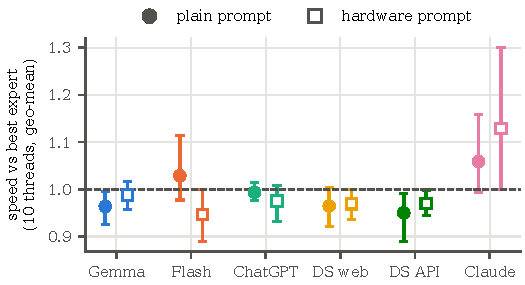
\includegraphics[width=\columnwidth]{figs/vs_best.pdf}
\caption{Speed of parallelization-only answers relative to the best expert schedule at 10 threads (geometric mean, 95\% bootstrap CI).}\label{fig:vsbest}
\end{figure}

The expert alternative recommended for asymmetric processors does not help on macOS: the AID-style calibrated split, which measures thread speed once and divides iterations proportionally~\cite{saez2020aid,beserra2026amp}, was slower than the best ordinary schedule on all \NumCalibKernels{} kernels where we applied it (by \NumCalibSlowerMin--\NumCalibSlowerMax\%). Because macOS migrates threads between core types, a split calibrated at start-up no longer matches where threads run.

\subsection{RQ3: Hardware-aware and explicit prompts}
Describing the hardware changes the code of two models and not the others. Paired by kernel and sample, Gemma switched \NumSwitchUpGemma{} answers from static to an adaptive schedule and none the other way (exact McNemar $p$\NumSwitchPGemma), and Claude \NumSwitchUpClaude{} ($p=\NumSwitchPClaude$); ChatGPT and DeepSeek on the web switched none, and the pinned DeepSeek API model, sampled three times per prompt, switched \NumSwitchUpDsapi{} and back \NumSwitchDownDsapi{} ($p=\NumSwitchPDsapi$). The speed of correct answers rose correspondingly for Gemma and Claude (paired Wilcoxon $p=\NumPGemma$ and $p=\NumPClaude$) and did not change for ChatGPT ($p=\NumPChatgpt$), DeepSeek web ($p=\NumPDeepseek$) or the DeepSeek API ($p=\NumPDsapi$). Asking explicitly for code that copes with the slower E-cores produced adaptive schedules in every Gemma answer but still no topology queries, and \NumShortcutNHwx{} correct answers took an algorithmic shortcut.

\subsection{RQ4: Measurement feedback}
Giving each model its own measured times (serial, 1, 4 and 10 threads) without naming a cause did not lead any model to the asymmetry. Of the \NumFbStaticTotal{} answer pairs that used a static schedule before feedback, \NumFbStaticToAdapt{} switched to an adaptive one. Among answers that stayed free of shortcuts, parallel scaling $S=T_1/T_{10}$ was unchanged or slightly worse ($\times$\NumFbScaleRatio, $p=\NumFbScaleP$), while speed relative to the expert improved by a factor of \NumFbBestRatio{} ($p=\NumFbBestP$), entirely through serial rewrites such as vectorization and tiling. Feedback also made shortcuts common: the share of correct answers that remove work rose from \NumShortcutPlain\% (plain) to \NumShortcutFb\% (Fig.~\ref{fig:feedback}), by folding repetitions into a multiplication, replacing trial division with a sieve, or caching Collatz chains. \NumFbBroken{} previously correct answers became incorrect and none were repaired.

\begin{figure}[t]\centering
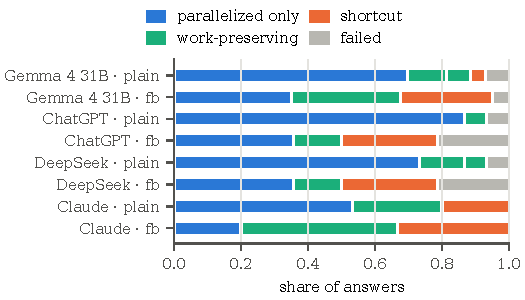
\includegraphics[width=\columnwidth]{figs/feedback.pdf}
\caption{What the answers did, before (plain) and after measurement feedback (fb).}\label{fig:feedback}
\end{figure}

\subsection{Oversubscription}
Running 20 threads on the 10 cores narrows the static penalty instead of widening it (Fig.~\ref{fig:oversub}): for mandelbrot the static/adaptive ratio falls from \NumOverMandelbrotTen{} to \NumOverMandelbrotTwenty, for trisum from \NumOverTrisumTen{} to \NumOverTrisumTwenty. Smaller static chunks plus OS time-slicing act as coarse load balancing.

\begin{figure}[t]\centering
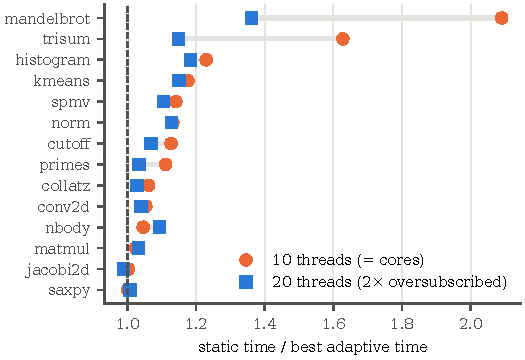
\includegraphics[width=\columnwidth]{figs/oversub.pdf}
\caption{Static time divided by best adaptive time at 10 threads and at 20 threads (expert code).}\label{fig:oversub}
\end{figure}

\subsection{Energy}
Using all cores with a good schedule is also the most frugal option: one mandelbrot run consumed \NumMandelJDyn\,J of CPU energy with \texttt{dynamic} on ten threads, against \NumMandelJStatic\,J with \texttt{static} and \NumMandelJSerial\,J serially.

\section{Discussion}
\textbf{Why LLM code mostly survives asymmetry.} The models do not reason about the hardware; none queried it in \NumAllAnswers{} answers. They avoid most of the cost by habit: for loops with visibly uneven work they almost always choose \texttt{dynamic} or \texttt{guided} (\NumAdaptIrregular\% of plain answers), and those are also the right choice on an asymmetric processor; for uniform loops they almost never do (\NumAdaptUniform\%). The residual cost lies where the habit and the hardware disagree: loops whose iterations are equally expensive look safe to statically partition, yet on the M4 equal chunks finish at unequal times once the fifth thread lands on an E-core.

\textbf{Why the textbook fix fails here.} Calibrated splits assume that a thread keeps its core. macOS gives no affinity control and moves threads between clusters (Fig.~\ref{fig:placement}), so a split measured at start-up is stale within the loop. On this platform, adaptive scheduling---or simply oversubscription---is more robust than static calibration.

\textbf{Why feedback does not help.} Measured times tell a model that its code is slow but not why. Without a hint about core types, every model looked for serial inefficiency, which on our kernels was often real, and frequently found it by removing repeated work. Optimization feedback for parallel code therefore needs to carry the hardware cause, or the evaluation must guard against shortcuts, as ours does with the $F\cdot S$ decomposition.

\textbf{Advice for practitioners.} On hybrid CPUs, prefer \texttt{dynamic} or \texttt{guided} schedules for every loop an LLM parallelizes, including uniform-cost ones; do not rely on describing the hardware in the prompt, since only some models act on it; avoid start-up-calibrated static splits on systems that migrate threads; and treat large speedups after optimization feedback as suspect until the algorithm is checked.

\section{Threats to Validity}
\textbf{One platform.} All measurements come from one Apple M4 laptop under macOS; Intel hybrid processors under Linux allow pinning and may behave differently. The mechanisms we identify (equal chunks on unequal cores, start-up calibration under migration) are platform-independent, but their magnitudes are not.
\textbf{Model versions.} Web chatbots do not report exact versions; the DeepSeek API runs pin a version and reproduce the web findings. Web answers are single samples, which limits per-model claims; API models were sampled three times.
\textbf{Prompt wording.} We used one wording per style. Other phrasings could change behaviour; the plain and hardware prompts differ only by the hardware paragraph, so their comparison is controlled.
\textbf{Measurement.} The fanless laptop could throttle during long runs. Configurations ran in shuffled order with cool-downs, and serial times measured on different nights agree within 1\% for \NumReproWithinOne{} of 15 kernels (at most \NumReproMaxDev\%). Low Power Mode, which slows single-thread runs on this machine by a factor of \NumLpmMin--\NumLpmMax, was off for all reported runs.
\textbf{Compiler.} One Apple clang miscompilation (histogram) was worked around by disabling vectorization for every histogram build, serial included, so that comparisons stay within one compiler configuration.
\textbf{Classification.} Shortcut and rewrite classes were assigned by reading code; the rules and per-answer labels are released for inspection.

\section{Conclusion}
LLMs parallelize loops for asymmetric P/E-core processors without ever considering that the cores differ. They lose little on irregular loops, where habit leads them to adaptive schedules, and up to \NumStaticUniMax\% on uniform loops, where habit leads them to static ones. Describing the hardware helps some models and not others; measurement feedback helps none with the asymmetry and makes shortcuts about \NumShortcutRatio{} times more common. Simple practices---adaptive schedules everywhere, or oversubscription---recover most of the loss, while start-up calibration does not survive thread migration on macOS. Our prompts, answers, timings, power logs and scripts are released to support replication on other hybrid processors.

\bibliographystyle{IEEEtran}
\bibliography{refs}
\end{document}
